\documentclass[tikz,border=8pt]{standalone}
\usepackage{amsmath,amssymb}
\usetikzlibrary{arrows.meta,automata,positioning,quotes}
\begin{document}
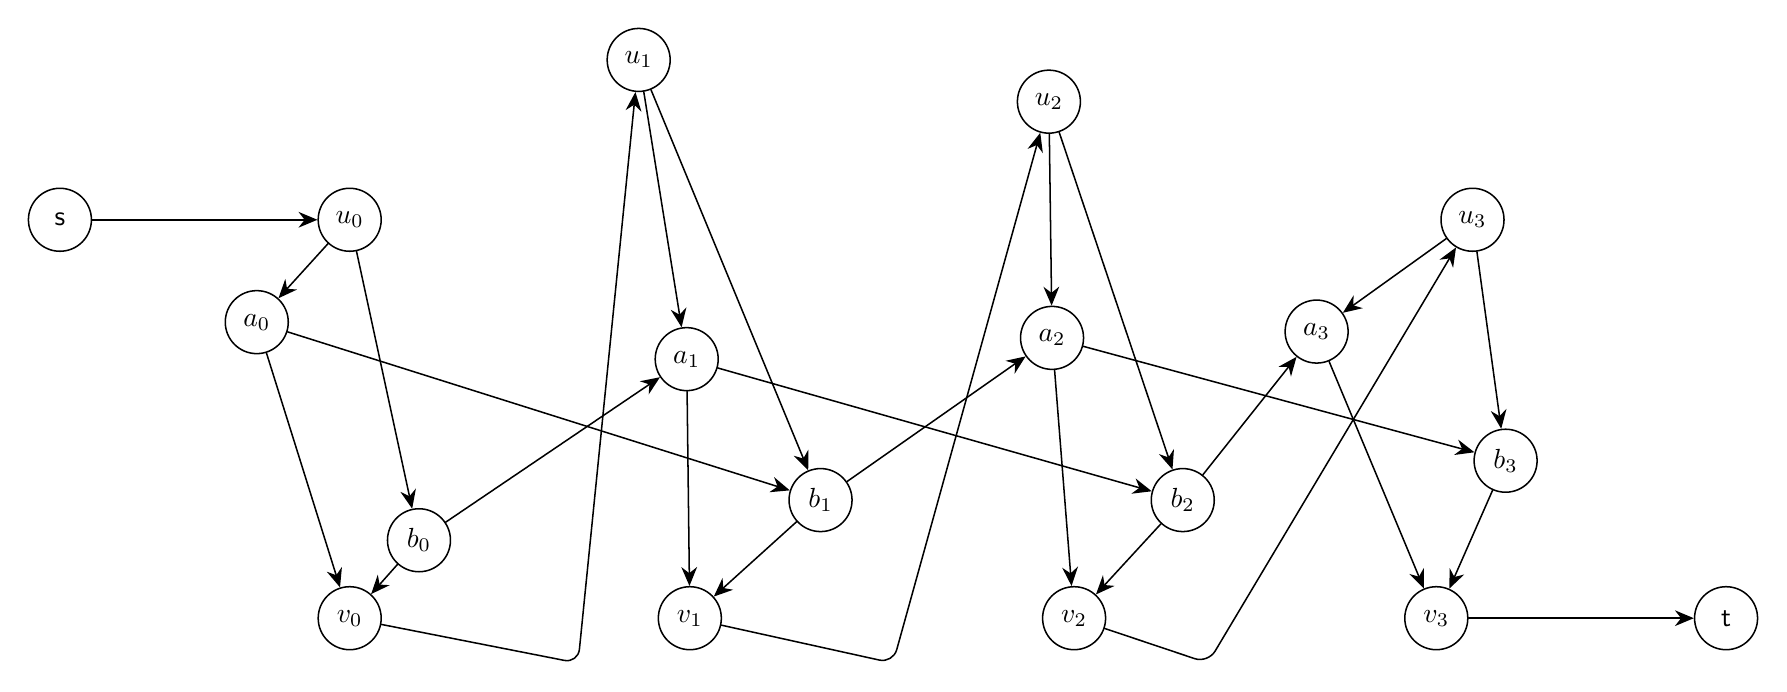
\begin{tikzpicture}[x=1cm,y=1cm]
\tikzset{
  graphnode/.style={circle,draw=black,line width=0.55pt,minimum size=8mm,inner sep=1pt,font=\sffamily},
  graphedge/.style={draw=black,line width=0.55pt,line cap=round,line join=round},
  directed/.style={graphedge,-{Stealth[length=2.4mm,width=2.0mm]}},
  undirected/.style={graphedge}
}
\node[graphnode] (n_s) at (-10.58,2.53) {s};
\node[graphnode] (n_t) at (10.58,-2.53) {t};
\node[graphnode] (n_u_0) at (-6.90,2.53) {$u_{0}$};
\node[graphnode] (n_v_0) at (-6.90,-2.53) {$v_{0}$};
\node[graphnode] (n_a_0) at (-8.08,1.23) {$a_{0}$};
\node[graphnode] (n_b_0) at (-6.02,-1.54) {$b_{0}$};
\node[graphnode] (n_u_1) at (-3.23,4.56) {$u_{1}$};
\node[graphnode] (n_v_1) at (-2.58,-2.53) {$v_{1}$};
\node[graphnode] (n_a_1) at (-2.62,0.76) {$a_{1}$};
\node[graphnode] (n_b_1) at (-0.92,-1.03) {$b_{1}$};
\node[graphnode] (n_u_2) at (1.98,4.03) {$u_{2}$};
\node[graphnode] (n_v_2) at (2.30,-2.53) {$v_{2}$};
\node[graphnode] (n_a_2) at (2.02,1.03) {$a_{2}$};
\node[graphnode] (n_b_2) at (3.68,-1.03) {$b_{2}$};
\node[graphnode] (n_u_3) at (7.36,2.53) {$u_{3}$};
\node[graphnode] (n_v_3) at (6.90,-2.53) {$v_{3}$};
\node[graphnode] (n_a_3) at (5.38,1.11) {$a_{3}$};
\node[graphnode] (n_b_3) at (7.78,-0.53) {$b_{3}$};
\draw[directed] (n_u_0) -- (n_a_0);
\draw[directed] (n_u_0) -- (n_b_0);
\draw[directed] (n_a_0) -- (n_v_0);
\draw[directed] (n_b_0) -- (n_v_0);
\draw[directed] (n_u_1) -- (n_a_1);
\draw[directed] (n_u_1) -- (n_b_1);
\draw[directed] (n_a_1) -- (n_v_1);
\draw[directed] (n_b_1) -- (n_v_1);
\draw[directed] (n_u_2) -- (n_a_2);
\draw[directed] (n_u_2) -- (n_b_2);
\draw[directed] (n_a_2) -- (n_v_2);
\draw[directed] (n_b_2) -- (n_v_2);
\draw[directed] (n_u_3) -- (n_a_3);
\draw[directed] (n_u_3) -- (n_b_3);
\draw[directed] (n_a_3) -- (n_v_3);
\draw[directed] (n_b_3) -- (n_v_3);
\draw[directed] (n_s) -- (n_u_0);
\draw[directed,rounded corners=5pt] (n_v_0) -- (-4.00,-3.10) -- (n_u_1);
\draw[directed,rounded corners=5pt] (n_v_1) -- (0.00,-3.10) -- (n_u_2);
\draw[directed,rounded corners=5pt] (n_v_2) -- (4.00,-3.10) -- (n_u_3);
\draw[directed] (n_v_3) -- (n_t);
\draw[directed] (n_a_0) -- (n_b_1);
\draw[directed] (n_b_0) -- (n_a_1);
\draw[directed] (n_a_1) -- (n_b_2);
\draw[directed] (n_b_1) -- (n_a_2);
\draw[directed] (n_a_2) -- (n_b_3);
\draw[directed] (n_b_2) -- (n_a_3);
\end{tikzpicture}
\end{document}
